\chapter{Multitask learning}

So far we have considered \ac{AES} and \ac{NLI} as independent tasks and run
separate experiments. We will now try to train models to predict both tasks
simultaneously.

In table \ref{tab:multitask-results}, we see the results of running some of
the most successful models from the previous chapter in a multi-task setting,
using the essay's L1 as the auxiliary label to predict. The number following
the model name is the weight given to the auxiliary loss during training.

In single task setup, the models performed as shown in table
\ref{tab:singletask-results}.

\begin{table}
  \centering
  \begin{tabular}{lrrrr}
    \toprule
            & \multicolumn{2}{c}{All labels}       & \multicolumn{2}{c}{Collapsed labels} \\
    \cmidrule(lr){2-3}
    \cmidrule(lr){4-5}
    Model & Macro \FI   & Micro \FI   & Macro \FI   & Micro \FI \\
    \midrule
    %       cnn-26094553_05             cnn-26094553_06
    CNN1  &     $0.235$ &     $0.382$ &     $0.404$ &    $0.699$ \\
    %       cnn-26094553_11             cnn-26094553_12
    CNN2  &     $0.255$ &     $0.447$ &     $0.393$ &    $0.740$ \\
    %       rnn-25858209                rnn-25858211
    RNN1  &     $0.354$ &     $0.390$ &     $0.493$ &    $0.724$ \\
    %       rnn-25985451                rnn-25985452
    RNN2  &     $0.277$ &     $0.407$ &     $0.624$ &    $0.756$ \\
    \bottomrule
  \end{tabular}
  \caption{CNN1: Static, pretrained embeddings size 50.
           CNN2: Static, pretrained embeddings size 50, POS as side input.
           RNN1: Attention model with GRU cell, dynamic pretrained
           embeddings size 50.
           RNN2: Attention model with LSTM cell, dynamic pretrained
           embeddings size 50, POS as side input.}
  \label{tab:singletask-results}
\end{table}

The reported metrics apply to the main task, CEFR prediction, only. It seems
that the auxiliary task is beneficial for all CNN models. All CNN models get
higher macro and micro \FI in the multi-task setup. Moreover, a higher weight
given to the auxiliary L1 prediction task seems to improve macro \FI
performance across the board. The effect of the auxiliary task weight seems
less clear on the micro \FI, but remember that in our setup, the micro \FI is
a side effect of the highest macro \FI seen during training.

\begin{table}
  \centering
  \begin{tabular}{lrrrr}
    \toprule
            & \multicolumn{2}{c}{All labels}       & \multicolumn{2}{c}{Collapsed labels} \\
    \cmidrule(lr){2-3}
    \cmidrule(lr){4-5}
    Model     & Macro \FI        & Micro \FI        & Macro \FI        & Micro \FI \\
    \midrule
    %           cnn-multi-26199963_1                  cnn-multi-26199963_2
    CNN1 0.25 &         $0.233$  &         $0.439$  &         $0.380$  &         $0.715$  \\
    %           cnn-multi-26199963_3                  cnn-multi-26199963_4
    CNN1 0.5  &         $0.246$  &         $0.398$  &         $0.389$  &         $0.732$  \\
    %           cnn-multi-26199963_5                  cnn-multi-26199963_6
    CNN1 0.75 &         $0.247$  &         $0.431$  &         $0.408$  &         $0.707$  \\
    \midrule
    %           cnn-multi-26199963_7                  cnn-multi-26199963_8
    CNN2 0.25 &         $0.259$  &         $0.455$  &         $0.406$  &         $0.764$  \\
    %           cnn-multi-26199963_9                  cnn-multi-26199963_10
    CNN2 0.5  &         $0.270$  &         $0.415$  &         $0.398$  &         $0.748$  \\
    %           cnn-multi-26199963_11                 cnn-multi-26199963_12
    CNN2 0.75 &         $0.275$  &         $0.463$  &         $0.414$  &         $0.780$  \\
    \midrule
    %           rnn-multi-26199963_13                 rnn-multi-26199963_14
    RNN1 0.25 &         $0.301$  &         $0.431$  &         $0.506$  &         $0.797$  \\
    %           rnn-multi-26199963_15                 rnn-multi-26199963_16
    RNN1 0.5  &         $0.333$  &         $0.472$  &         $0.529$  &         $0.772$  \\
    %           rnn-multi-26199963_17                 rnn-multi-26199963_18
    RNN1 0.75 &         $0.283$  &         $0.488$  &         $0.526$  &         $0.772$  \\
    \midrule
    %           rnn-multi-26199963_19                 rnn-multi-26199963_20
    RNN2 0.25 &         $0.320$  &         $0.423$  &         $0.565$  &         $0.683$  \\
    %           rnn-multi-26199963_21                 rnn-multi-26199963_22
    RNN2 0.5  &         $0.292$  &         $0.447$  &         $0.533$  &         $0.772$  \\
    %           rnn-multi-26199963_23                 rnn-multi-26199963_24
    RNN2 0.75 &         $0.285$  &         $0.447$  &         $0.428$  &         $0.805$  \\
    \bottomrule
  \end{tabular}
  \caption{CNN1: Static, pretrained embeddings size 50.
           CNN2: Static, pretrained embeddings size 50, POS as side input.
           RNN1: Attention model with GRU cell, dynamic pretrained
           embeddings size 50.
           RNN2: Attention model with LSTM cell, dynamic pretrained
           embeddings size 50, POS as side input.}
  \label{tab:multitask-results}
\end{table}

For the RNNs, the results are not quite as clear. The multi-task models were
not able to exceed the macro \FI scores of $0.354$ (all labels) and $0.624$
(collapsed labels), but this may be because the macro \FI metric is unstable
because of the `A2' class with one single example in the dev set. For the
same models, accuracy did increase in the multitask setup.

The model `RNN1 0.5' was the best performing multitask model by several
metrics. In addition to macro \FI, it was the best model in terms of RMSE
($0.888$), Pearson correlation coefficient ($0.765$) and Spearman's ranked
correlation coefficient ($0.768$).


\begin{figure}
  % cnn-multi-26199963_11
  \centering
  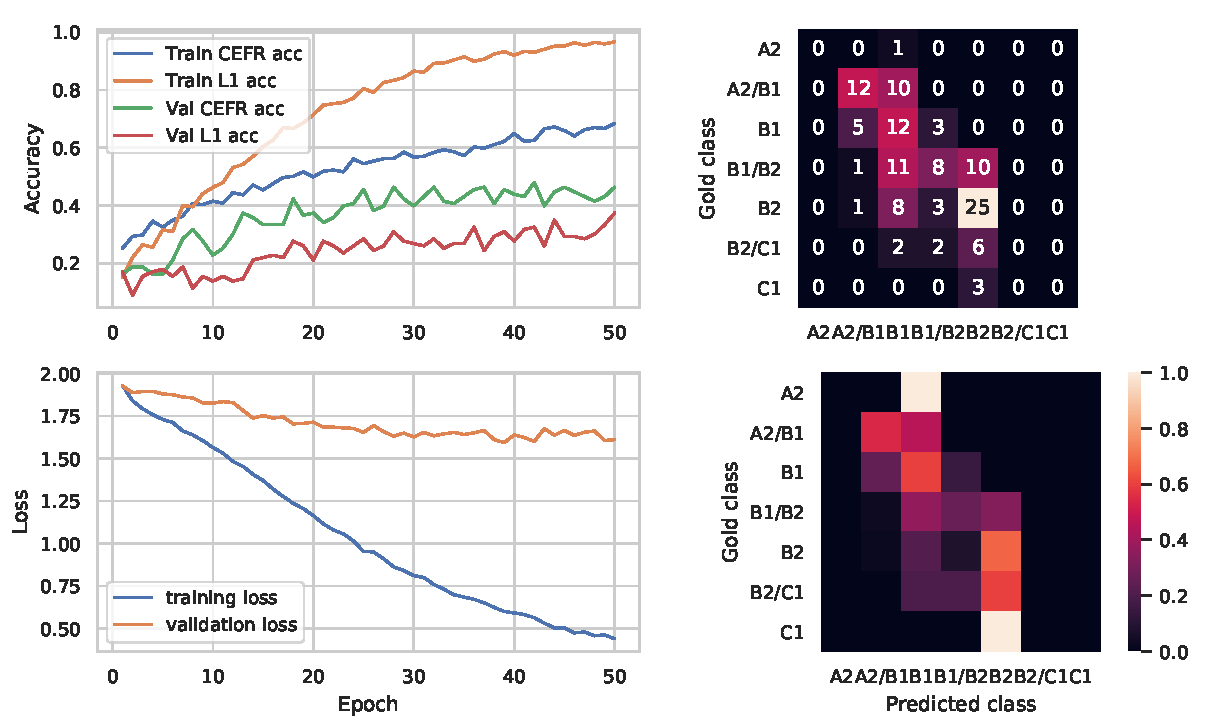
\includegraphics[width=\textwidth]{cnn-multi-training}
  \caption{CNN2 0.75. Training and validation loss and accuracy over 50 epochs of training.
           Also, confusion matrices with counts and normalized by class.}
  \label{fig:cnn-multi-training}
\end{figure}


\begin{figure}
  % rnn-multi-26199963_15
  \centering
  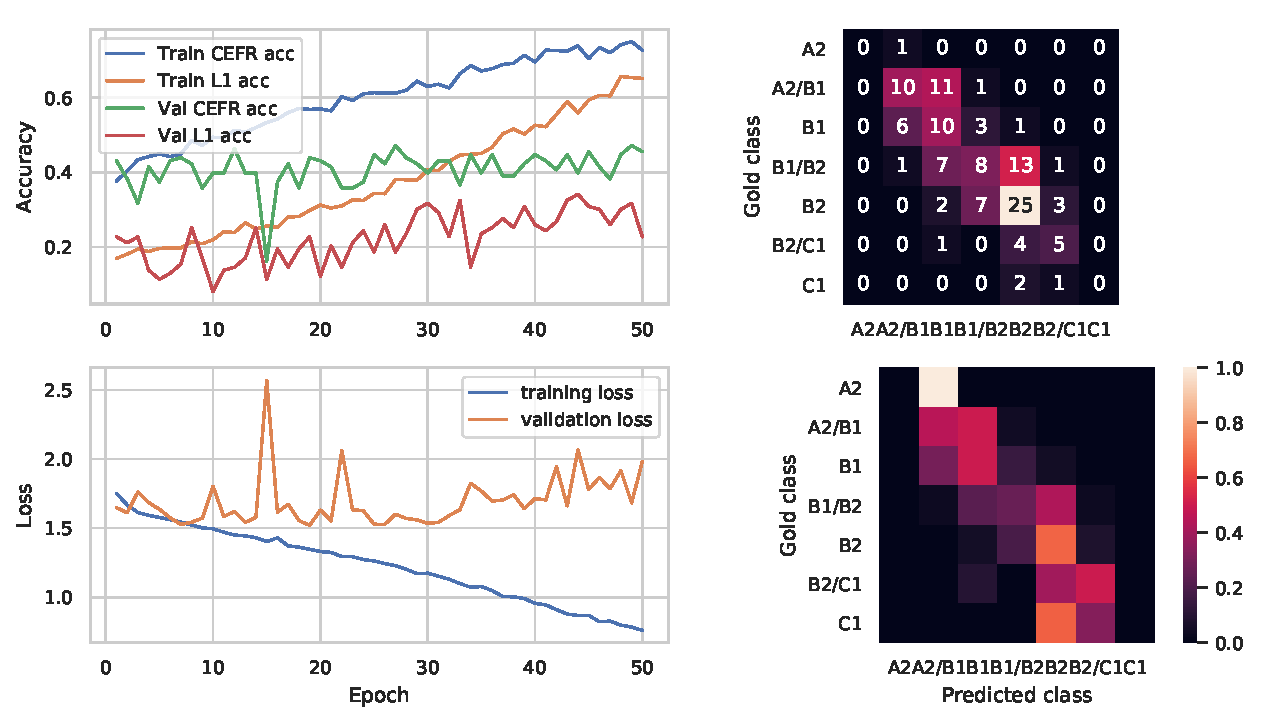
\includegraphics[width=\textwidth]{rnn-multi-training}
  \caption{RNN1 0.5. Training and validation loss and accuracy over 50 epochs of training.
           Also, confusion matrices with counts and normalized by class.}
  \label{fig:rnn-multi-training}
\end{figure}
